\documentclass[11pt]{article}
\usepackage{graphicx}
\usepackage[margin=1in]{geometry} %reducir márgenes
\usepackage{cite} %opciones entre {}
\pagestyle{empty} %quitar números de página
\usepackage{amsmath, amssymb, amsfonts} %paquete para escribir con un formato matematico
\usepackage{enumerate}

\setlength{\parskip}{8mm} %configurar opcion entre parrafos dejar una linea
\parindent 0ex %no sangrado al empezar parrafos
\renewcommand{\baselinestretch}{1.2} 

\begin{document}

\section*{ \textbf{Problema n-alcanos para estimar la dieta de los herbívoros} } %definir estilo de la función
A continuación vamos a resumir el problema planteado en el artículo \cite{n-alkanes_problem} escrito por P.Barcia, M. N. Bugalho, M. L. Campagnolo y J. O. Cerdeira. 

Los n-alcanos son hidrocarburos que se encuentran en las cutículas de las plantas, y que pueden ser usados para estimar la composición de la dieta de herbívoros a partir de la composición de sus heces. Una limitación del uso de n-alcanos es que para realizar esta estimación por medio de procedimientos matemáticos, el número de marcadores (i.e. diferentes n-alcanos que se pueden detectar en las heces de un animal) debe ser mayor que el número de plantas diferentes incluidas en la dieta. En este caso tratamos con herbívoros en libertad que se alimentan de plantas complejas. Para ello usaremos un enfoque para estimar la dieta con n-alcanos que se aplica en todos los casos.

El modelo usa programación lineal para estimar el mínimo y el máximo de las proporciones de cada planta de la dieta. Se ilustra el modelo con dos conjuntos de datos de plantas y heces, obtenidos en experimentos de pastoreos de ovejas en Australia y el estudio de ciervos rojos en Portugal. En estos experimentos podemos ver qué proporciones de sustancias forman parte de la dieta de estos dos tipos de animales. (no hablaremos en este artículo de los beneficios que trae este estudio, permitiéndonos añadir sustancias beneficiosas para los animales en plantas que comen o eliminar otras que sean perjudiciales para su salud.)

\subsection{Introducción}

Conocer la composición de la dieta de los herbívoros es importante para comprender su ecología y alimentación, lo cual es útil para medir sus efectos sobre la vegetación y los ecosistemas.

Las especies de plantas se caracterizan por diferentes concentraciones de n-alcanos. Los marcadores químicos recuperados en las heces pueden ser utilizados para cuantificar las plantas ingeridas por un animal.

A partir del estudio de Dove y Mayes (1991), se planteó resolver el problema con un sistema restringido de ecuaciones lineales. 

El requisito de que el número máximo de componentes que se pueden detectar en la dieta está limitado por el número de marcadores disponibles es común en todos los casos. En el caso donde haya más plantas que n-alcanos. Se trata de agrupar las plantas en grupos bien definidos funcionalmente (por ejemplo, pastor, leguminosas, ramoneo) o estadísticamente.

Al ser nuestro objetivo estimar la composición de la dieta de animales herbívoros en libertad a partir de n-alcanos. Donde el número de las especies de plantas va a ser siempre superior a los n-alcanos. Es importante realizar grupos coherentes de especies.\\
Describimos un modelo en el que la composición de la dieta se identifica con (posibles) infinitas combinaciones de especies. Los límites superior e inferior de las concentraciones de cada especie  en la dieta pueden determinarse mediante programación lineal. El enfoque se puede aplicar sin importar si el número de marcadores es menor, igual o mayor que el número de especies, evitando así la necesidad de agrupar especies\\
Probamos el modelo en dos conjuntos de datos que constan de
registros de los perfiles de n-alcanos de diferentes especies de plantas y heces de ovejas y ciervos recolectadas en experimentos llevados a cabo en Australia y Portugal. 

\subsection{Material y métodos}

Supongamos que $d$ es el número de n-alcanos en planta y hez. Cada hez de la muestra puede ser considerada un \textbf{punto} en el espacio d-Euclideo, que describe la concentración de cada d n-alcanos. Cada especie de planta puede ser interpretada como un vector en este espacio. Definiendo el valor de cada $d$ n-alcano en la planta (Figura \ref{fig:espacio01}).

\begin{figure}[h!] 
\centering
    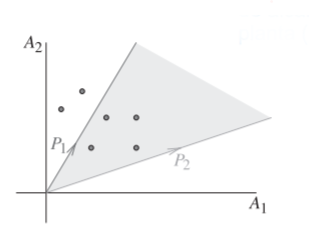
\includegraphics[width=0.4\textwidth]{espacio01.png}
\caption{Ejemplo representa dos alcanos ($A_1$,$A_2$), dos especies de plantas (vectores $P_1$ y $P_2$), y seis muestras de heces (puntos de la figura). El área sombreada es el cono bidimensional generado por los vectores $P_1$ y $P_2$.}
\label{fig:espacio01}
\end{figure}

Las dietas son combinaciones lineales, es decir, las sumas ponderadas de los vectores representan las especies vegetales. El peso o coeficiente de cada vector define la cantidad correspondiente de la especie en la dieta. Cada coeficiente dividido  por el sumatorio de los coeficientes, da la proporción de cada planta en la dieta. Si $P_1, P_2, ..., P_p$ son los d-vectores que representan p plantas, cada vector indica la concentración de n-alcanos en esa especie, la combinación lineal con coeficientes $c_1,c_2, ... , c_p$ es $c_1 P_1 + c_2 P_2 + ... + c_p P_p$. \\
Las combinaciones lineales con coeficientes negativos son \textit{"dietas sin sentido"}. Por lo tanto, debemos centrar nuestra atención en las combinaciones lineales que tienen coeficientes no negativos. Este conjunto de combinaciones lineales no negativas forma el cono generado por esos dos vectores. En la Figura \ref{fig:espacio01} el cono generado por los vectores $P_1$ y $P_2$ es la región sombreada. Usamos $C$ para denotar el cono generado, es decir: $$ C = { c_1 P_1 + c_2 P_2 + ... + c_p P_p, \text{ con } c_1,c_2,...,c_p >=0} $$

La estimación de dietas a partir de pruebas fecales $F_1, F_2, ... . F_q $ toma una muestra $F$ y buscar sí:

\begin{enumerate}[(i)]
\item $F$ pertenece al cono $C$ o
\item $F$ es un punto fuera de $C$.
\end{enumerate}

Esto es determinado resolviendo el sistema de ecuaciones linear $$Ax=F.$$

Donde A es $d \times p$ cuyas columnas son los vectores $P_1, P_2 , ... , P_p$ que representan las plantas. Si todos los componentes de la solución $x$ son no-negativos, estaremos en el caso (i), y $x$ especifica la composición correspondiente de especies en las heces. Si hay un componente negativo, estamos en la situación (ii), indicando que son \textit{"dietas sin sentido"}. Esto puede resultar de errores en la medición de las concentraciones de n-alcanos, o la existencia de plantas no incluidas en la muestra. Una posible solución es encontrar un vector no negativo de coeficientes que se aproximen a la $x$. Un posible enfoque consiste en:

\begin{enumerate}[(i)]
\setcounter{enumi}{2}
\item identificar un punto $F_0$ en el cono $C$ considerado \textit{"similar a"} $F$, y
\item usando $F_0$ en lugar de $F$, proceder resolviendo como en (i) el sistema de ecuaciones (S).
\end{enumerate}

Normalmente la proyección de $F$ en $C$, es decir el punto en $C$ más cercano a $F$, es seleccionado para ser $F_0$. En la figura \ref{fig:espacio01} hay dos puntos en el caso (ii). Cada uno será remplazado por su proyección en $C$, por lo que se encontrará definido por el vector $P_1$.
La dieta estimada del animal se calcula finalmente a partir de las soluciones obtenidas de las muestras fecales $F_1,F_2,...,F_q$.
A menudo, la dieta es definida por el promedio de las $q$ soluciones, es decir, la dieta son las soluciones del sistema de ecuaciones lineal ($S$).

En este ejemplo estamos asumiendo que el número de n-alcanos es igual al número de especies de plantas, es decir, que $A$ es una matriz cuadrada (no-singular). Si hubiera más n-alcanos que especies la situación no cambiaría (Figura \ref{fig:espacio02}). Pero si hubiese más plantas que n-alcanos (Figura \ref{fig:espacio03}) la situación cambia considerablemente. Ahora cualquier combinación lineal no-negativa de vectores $P_1$ y $P_3$ define un nuevo vector $P$ contenido en el cono generado por estos vectores. Cualquier punto $F$ encontrado en el cono formado por $P$ y $P_2$ es una combinación lineal no negativa de $P$ (en consecuencia de $P$ y $P_3$) y $P_2$. Al ser infinitos los vectores $P$ definidos a partir $P$ y $P_3$ tales que $F$ esta dentro del cono generado en $P$ y $P_2$, el sistema ($S$) puede tener un número infinito de soluciones no negativas. O lo que es lo mismo, la concentración de n-alcanos en las muestras fecales puede resultar de infinidad de mezclas de plantas diferentes.

\begin{figure}[h!] 
\centering
    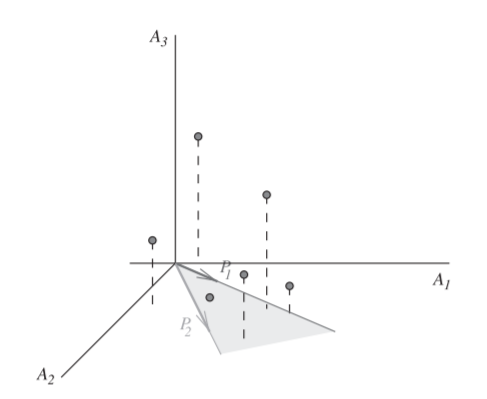
\includegraphics[width=0.4\textwidth]{espacio02.png}
\caption{Ejemplo representa tres n-alcanos ($A_1$,$A_2$,$A_3$), dos especies de plantas (vectores $P_1$ y $P_2$), y seis muestras de heces (puntos de la figura), dando lugar a un cono bidimensional generado por los dos vectores de plantas.}
\label{fig:espacio02}
\end{figure}

Por tanto, siempre que el número de especies supere al número de n-alcanos se suele enfocar el problema agrupando las especies en categorías. Sin embargo, no existe un claro criterio satisfactorio para decidir como agrupar las especies (cómo definir una partición $d$ al conjunto de vectores $P_1, P_2,...,P_p$) ni cómo ponderarlas dentro de cada grupo.

Para resolver este problema se sugiere un enfoque alternativo que usa números arbitrarios de especies de plantas y n-alcanos.

\begin{figure}[h!] 
\centering
    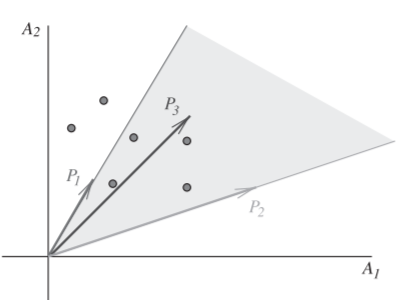
\includegraphics[width=0.4\textwidth]{espacio03.png}
\caption{Ejemplo representa dos n-alcanos ($A_1$,$A_2$), tres especies de plantas (vectores $P_1$, $P_2$ y $P_3$), y seis muestras de heces (puntos de la figura). El área sombreada es el cono bidimensional generado por los vectores $P_1$, $P_2$ y $P_2$..}
\label{fig:espacio03}
\end{figure}

Partiendo de $P_1, P_2,...,P_p$ vectores de $d$ representan $p$ potenciales plantas, donde $d$ es el número de n-alcanos usados, y $C$ el cono generado por los vectores, Denotamos $F_i = 1,2,...,q$ la proyección en $C$ del punto en $d$, y definimos $\phi$ como el conjunto de muestras fecales \textit{"correctas"}.

Definimos una dieta factible aquella solución no negativa del sistema lineal $Ax=F$, para cualquier punto de $F$ en $\phi$, donde $A$ es $d \times p$ matriz con columnas $P_1, P_2,...,P_p$. Hay muchas dietas factibles. No obstante, el conjunto de dietas está acotado por \textbf{límites superiores e inferiores}, la programación lineal es una herramienta adecuada para abordar algunas de las siguientes cuestiones sobre la dieta:

\begin{itemize}
    \item ¿Cuáles son las proporciones máximas y mínimas de cada especie en la dieta?
    \item ¿Cuáles son las proporciones máximas y mínimas de cada grupo en la dieta?
    \item ¿Cuál es la proporción mínima de una planta, en concreto  en aquellas dietas que cumplen un requisito ( por ejemplo, los niveles de ingesta de nitrógeno o tanino contenido)
\end{itemize}

En particular, Si $x_p$ denota el componente de $x$ correspondiente a la plata $P$, entonces $M(i,P) = \max\{x_p, \text{ sujeto a } A_x = F_i \text{ y } x>=0\}$ y $m(i,P) = \min\{x_p, \text{ sujeto a } A_x=F_i \text{ y } x>=0\}$, for $i = 1,2,...,q$, nos permite responder a las preguntas sobre la presencia o ausencia de las especies vegetales en la dieta.

\begin{itemize}
    \item Especies nunca se comen - especies ausentes (absent species)
    \item Especies se comen siempre - especies obligatorias (mandatory species)
    \item Especies identificables en algunas muestras fecales - especies obligatorias condicionales (conditional mandatory species)
\end{itemize}

En caso de que la especie vegetal no coincida con ninguna de las categorías anteriores (especies opcionales) no podemos asegurar si se comen o no, sería necesario realizar más recopilación de datos en busca de esa especie no encontrada.

\textbf{Especies ausentes} (Absent species): son las plantas no incluidas en ninguna dieta. La especie $P$ está ausente si el correspondiente coeficiente en cada solución no negativa de la ecuación $A_x=F$, para cada $F$ en $\phi$, \textit{es igual a 0}. Esto puede determinarse comprobando $M(i,P) = 0, \text{ for } i =1,2,...,q$. Este caso coincidirá con los vectores $P$ que no permiten llegar a una muestra.

\textbf{Especies obligatorias} (Mandatory species): son las presentes en todas la dietas. La especie $P$ es obligatoria en el coeficiente de cada solución no negativa.$A_x=F$, por cada F en $\phi$, \textit{es mayor que 0}. Desde un punto de vista geométrico, $P$ es obligatorio si no hay $F_i$ en el cono $C_p$. Para decidir si una especie es obligatoria tenemos que comprobar si $m(iP)>0, \text{ for } i = 1,2,...,q$. Son obligatorias las muestras que se encuentren justo en el vector de la especie.

\textbf{Especies obligatorias condicionales} (Conditional mandatory species): son las plantas obligatorias para algunas dietas pero no para todas. La especie $P$ es condicional obligatoria si para algunos es obligatoria y para otros no. $F$ en $\phi$ no hay soluciones no negativas en $A_x=F$ con coeficiente correspondiente a $P$ igual a $0$. Equivalentemente, especies $P$ son condicional obligatorias si hay puntos en $\phi$ que están en $C_p$, y otros que no. Para comprobar si las especies son condicionales obligatorias tenemos que pasar en alguna $i=1,2,...,q, m(i,P)>0$. 

\textbf{Especies opcionales} (Optional species): son las plantas que no coinciden con ninguno de los casos anteriores. Especies $P$ son opcionales si para cada $F$ en $\phi$ hay soluciones no-negativas de $A_x=F$ para que el coeficiente $P$ sea igual a $0$, al menos para el lado derecho de $F$ existe una solución no negativa, para cuyo coeficiente de $P$ es mayor que $0$. La especie $P$ es opcional si ($P$ no está ausente y) $F$ está contenida en $C_p$. Si especie $P$ es opcional entonces $m(i,P)=0, \text{ para cada } i=1,2,...,q$ y $M(i,P)>0$, para al menos una $i$. 
Las especies opcionales son las únicas de las que no podemos asegurar si comieron o no determinadas plantas. Por lo tanto, puede ser interesante identificar un subconjunto de plantas de tamaño mínimo sin especies opcionales, Generando un cono que contiene $F$ (problema entero mixto - Programación lineal).

En la Figura \ref{fig:eje_prac} se muestra un ejemplo aplicando el modelo explicado anteriormente sobre un conjunto de datos sobre un rebaño de ovejas en Australia.

\begin{figure}[h!] 
\centering
    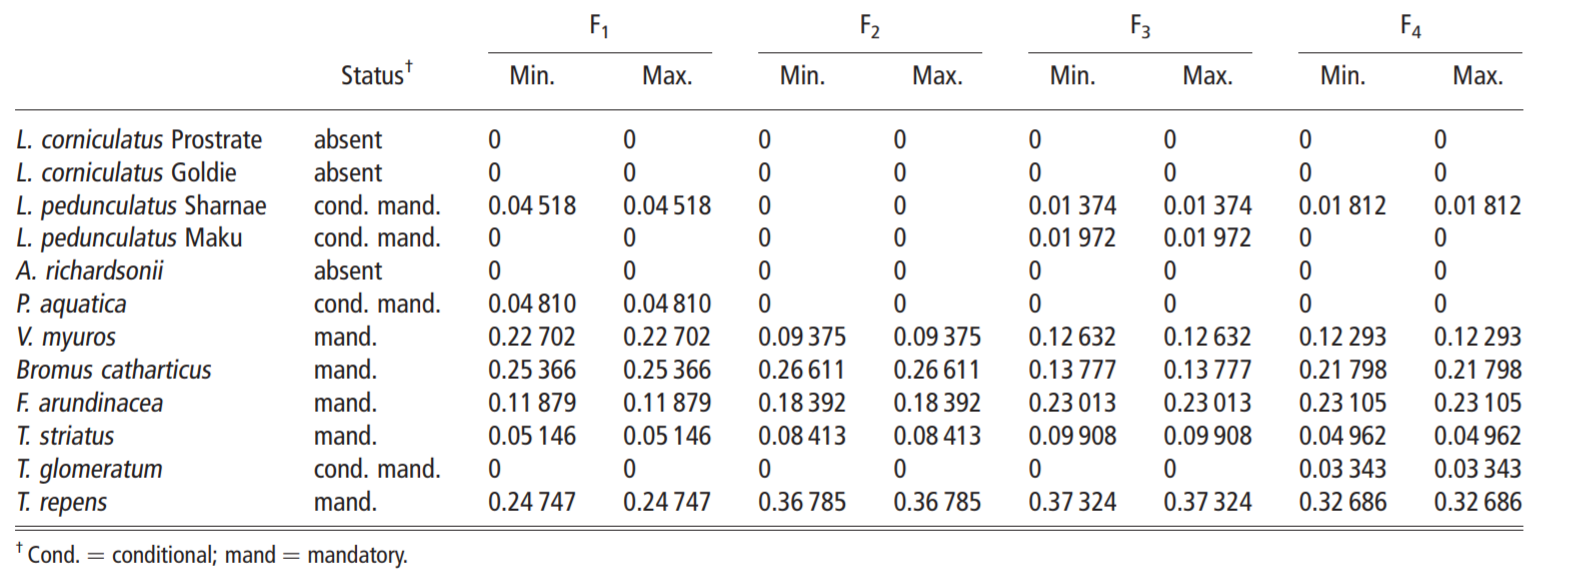
\includegraphics[width=1\textwidth]{resultados_ovejas.png}
\caption{Resultado de aplicar el modelo anterior sobre un conjunto de datos de ovejas en Australia, clasificando las especies de plantas y dando limites máximos y mínimos para las muestras fecales.}
\label{fig:res_ovej}
\end{figure}

\subsection{Ejercicio a mano:}
A continuación vamos a plantear la ecuación que nos permite calcular los n-alcanos que consumieron un determinado conjunto de animales. Para este ejemplo vamos a trabajar con dos especies de plantas ($p$),y dos tipos de n-alcanos ($d$).

$P_1$= $\{0.3,0.4\}$ tiene 0.3 del primer n-alcano y 0.4 del segundo n-alcano. \\
$d=2$ es el número de n-alcanos que definen las plantas.
\Large
$$P_1 = \{ 0.3 , 0.4 \} = \bigl[\begin{smallmatrix} 0.3\\ 0.4\end{smallmatrix}\bigr]$$
$$P_2 = \{ 0.1 , 0 \} = \bigl[\begin{smallmatrix} 0.1\\ 0\end{smallmatrix}\bigr]$$
\normalsize

Y los gramos de cada planta:
$$x_1\:gramos\:de\:P_1$$
$$x_2\:gramos\:de\:P_2$$


Partiendo de la ecuación definida anteriormente $Ax=F$ sabemos que $A$ es $\bigl[\begin{smallmatrix} P_1 & P_2\end{smallmatrix}\bigr]x=F$. E introduciendo los valores de este ejemplo obtenemos:

\LARGE
$$\bigl[\begin{smallmatrix} 0.3 & 0.1\\ 0.4 & 0 \end{smallmatrix}\bigr] \bigl[\begin{smallmatrix} x_1\\ x_2\end{smallmatrix}\bigr] = \bigl[\begin{smallmatrix} f_1\\ f_2\end{smallmatrix}\bigr]$$
$$\bigl[\begin{smallmatrix} 0.3\\ 0.4\end{smallmatrix}\bigr] x_1 + \bigl[\begin{smallmatrix} 0.1\\ 0\end{smallmatrix}\bigr] x_2  = \bigl[\begin{smallmatrix} f_1\\ f_2\end{smallmatrix}\bigr]$$
\normalsize

$$F_1 = \bigl[\begin{smallmatrix} 0.3\\ 0.2 \end{smallmatrix}\bigr] \:,\: F_2 = \bigl[\begin{smallmatrix} 0.1\\ 0 \end{smallmatrix}\bigr] \:,\: F_3 = \bigl[\begin{smallmatrix} 0\\ 0.2 \end{smallmatrix}\bigr]$$

Las $F$ son las muestras fecales, partiendo de $F_2$ que no tiene el segundo n-alcano, se puede deducir que $F_2$ \textbf{no} puede haber ingerido de $P_1$ (al tener $P_1$ gramos del primer n-alcano). En cuanto a $F_3$ no tiene al primer n-alcano. Por tanto, no puede haber ingerido ninguna de las especies vegetales, al tener todas valores del primer n-alcano $> 0$.

En la ecuación anterior para calcular $F_2$ $x_1$ tendría que valer $= 0$ y $x_2$ exactamente $1$, ya que $F_2$ coincide con la cantidad de n-alcanos de $P_2$.
\LARGE
$$\bigl[\begin{smallmatrix} 0.3\\ 0.4\end{smallmatrix}\bigr] 0 + \bigl[\begin{smallmatrix} 0.1\\ 0\end{smallmatrix}\bigr] 1  = F_2$$
\normalsize

\begin{figure}[h!] 
\centering
    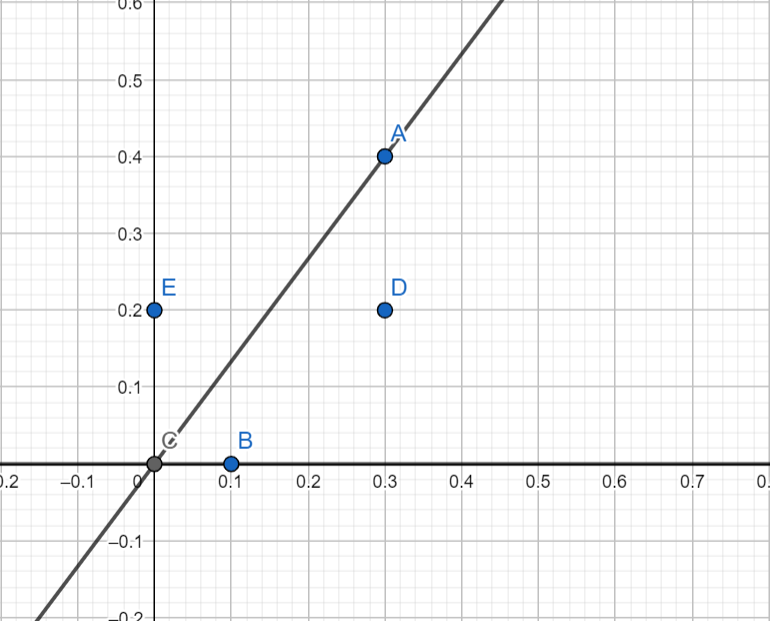
\includegraphics[width=0.5\textwidth]{ejemplo_practico.png}
\caption{En esta imagen podemos apreciar los vectores que pasan por A y B (que son las especies vegetales) y los puntos B y D (son muestras fecales que se pueden formar a partir de combinaciones entre estas dos plantas), en cuanto al punto E se desconoce de que especies puede provenir el número de n-alcanos encontrado.
}
\label{fig:eje_prac}
\end{figure}

\bibliographystyle{plain}
\bibliography{library}


\end{document}